\subsection{分岐は高々1つであること}

\begin{lemma}
  \label{lem:exist_two_extra_neighbors}
  \lean{exist_two_extra_neighbors}
  \leanok
  \uses{}
  $i, w \in V$で$3 \le \deg(i)$とする．
  このとき，$a, b \in V$で，以下すべてを満たすものが存在する：
  \begin{equation}
    a \ne b,\ a \ne w,\ b \ne w,\quad a \in N(i),\ b \in N(i).
  \end{equation}
  つまり，頂点$i$は頂点$w$の他に少なくとも$2$つの頂点$a, b$と隣接している．
\end{lemma}

\begin{proof}
  $S = N(i) \setminus\{w\}$とする．
  このとき，
  \begin{align}
    \# S
    &= \# N(i) - \# \{w\} \\
    &= \deg(i) - 1 \\
    &\ge 3 - 1 \\
    &= 2
  \end{align}
  である．
  よって，$a, b \in S$で$a \ne b$となるようなものがとれる．
  したがって，$S$の定め方より$a \ne b$以外の主張もすべて満たす．
\end{proof}

\begin{lemma}
  \label{lem:not_posDef_of_two_branches}
  \lean{not_posDef_of_two_branches}
  \leanok
  \uses{lem:dynkinGraph_preconnected, lem:exist_two_extra_neighbors}
  $C$はGCMでindecomposableであるとする．
  また，$u, v \in V$で$u \ne v$とし，$3 \le \deg(u),\ 3 \le \deg(v)$を満たすとする．
  このとき，$S(C)$は正定値でない．
\end{lemma}

\begin{proof}
  補題~\ref{lem:dynkinGraph_preconnected}より，$C$のDynkin graphは連結であるから$u$と$v$を結ぶ単純道$P = (u = p_0, p_1, \ldots, p_\ell = v)$がある．
  $u \ne v$であるから$1 \le \ell$である．
  $w_1 = p_1$とする．
  すると，$u$と$w_1$は隣接している．
  $3 \le \deg(u)$であるから補題~\ref{lem:exist_two_extra_neighbors}より，以下を満たす$a_1, a_2 \in V$がとれる：
  \begin{equation}
    a_1 \ne a_2,\ a_1 \ne w_1,\ a_2 \ne w_1,\ a_1 \ne u,\ a_2 \ne u,\quad C_{u a_1} \ne 0,\ C_{u a_2} \ne 0.
  \end{equation}
  すなわち，$u$は$3$つ以上の頂点と隣接しているから，そのうち$w_1, a_1, a_2$を相異なるようにとれる．
  全く同様に，$w_2 := p_{\ell - 1}, b_1, b_2$をとる：
  \begin{equation}
    b_1 \ne b_2,\ b_1 \ne w_2,\ b_2 \ne w_2,\ b_1 \ne u,\ b_2 \ne u,\quad C_{u b_1} \ne 0,\ C_{u b_2} \ne 0.
  \end{equation}
  今，以下のような状況である：
  \begin{figure}[h]
    \begin{center}
      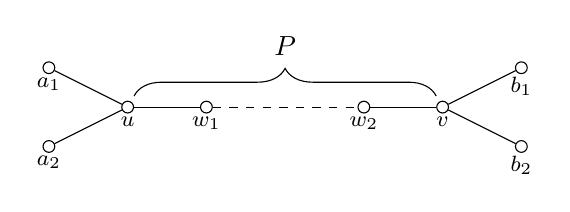
\begin{tikzpicture}[scale=1]
        % D_n
        \foreach \i in {2,3,5,6}
					\node[circle, draw, fill=white, inner sep=1.5pt] (\i) at (\i,-5.5) {};
				\foreach \i in {2,5}
					\draw (\i) -- (\the\numexpr\i+1\relax);
				\draw[dashed] (3) -- (5);
				\node[circle, draw, fill=white, inner sep=1.5pt] (0) at (1,-5) {};
				\node[circle, draw, fill=white, inner sep=1.5pt] (1) at (1,-6) {};
        \node[circle, draw, fill=white, inner sep=1.5pt] (7) at (7,-5) {};
				\node[circle, draw, fill=white, inner sep=1.5pt] (8) at (7,-6) {};
				\foreach \i in {0,1}
					\draw (\i) -- (2);
        \foreach \i in {7,8}
					\draw (\i) -- (6);
        \node[below] at (0) {\footnotesize $a_1$};
        \node[below] at (1) {\footnotesize $a_2$};
        \node[below] at (2) {\footnotesize $u$};
        \node[below] at (3) {\footnotesize $w_1$};
        %\node[below] at (4) {\footnotesize $5$};
        \node[below] at (5) {\footnotesize $w_2$};
        \node[below] at (6) {\footnotesize $v$};
        \node[below] at (7) {\footnotesize $b_1$};
        \node[below] at (8) {\footnotesize $b_2$};
        \draw [decorate,decoration={brace,amplitude=10pt, raise=4pt}]
        (2) -- (6) node[above, midway, yshift=15pt] {$P$}; %カッコ
      \end{tikzpicture}
    \end{center}
  \end{figure}

  $x := \transpose{(x_1, x_2, \ldots, x_n)} \in \R^n$を以下で定める：
  \begin{equation}
    x_i = \begin{cases}
      2, & i \in P,\\
      1, & i \in \{a_1, a_2, b_1, b_2\},\\
      0, & \textrm{otherwise}.
    \end{cases}
  \end{equation}
  $x_u = 2$であるから$x \ne 0$であり，定義から明らかに$0 \le x_i$である．

  補題~\ref{lem:quadform_nonpos_of_neighbor_bound}が使いたい．
  そこで，$0 < x_i$として，以下を示す：
  \begin{equation}
    2 x_i \le \sum_{j \in N(i)} x_j.
  \end{equation}

  $i = u$のとき，
  \begin{align}
    2 x_u
    &= 2 \cdot 2 \\
    &= 2 + 1 + 1 \\
    &=  \sum_{j \in \{w_1, a_1, a_2\}} x_j \\
    &\le \sum_{j \in N(u)} x_j
  \end{align}
  である．
  最後の等号は，$w_1, a_1, a_2$が相異なることから従う．
  最後の不等号は，$\{w_1, a_1, a_2\} \subseteq N(u)$と，$j \in N(u) \setminus \{w_1, a_1, a_2\}$に対し，$0 \le x_j$であることから従う．

  $i = v$のときも，$\{w_2, b_1, b_2\}$で考えれば全く同様にしてわかる．

  $i \in P \setminus \{u, v\}$のとき，$i \in P$であるから，$k \in I$を用いて$i = p_k$と表せる．
  $i \ne u = p_0,\ i \ne v = p_\ell$であるから，$0 < k < \ell$である．
  このとき，以下が成り立つことを示す：
  \begin{equation}
    p_{k-1}, p_{k+1} \in P,\qquad
    p_{k-1}, p_{k+1} \ne i,\qquad
    C_{i p_{k-1}}, C_{i p_{k+1}} \ne 0.
  \end{equation}
  $p_{k-1}, p_{k+1} \in P$は明らかである．
  今，$i = p_k$であるから$p_k$と$p_{k \pm 1}$との関係を調べれば良い．
  $k \pm 1, k < \ell$であるから$p_k$と$p_{k\pm1}$は隣接している．
  よって，後の2つも成り立つ．
  したがって，
  \begin{align}
    2 x_i
    &= 2 \cdot 2 \\
    &= 2 + 2 \\
    &= \sum_{j \in \{p_{k-1}, p_{k+1}\}} x_j \\
    &\le \sum_{j \in N(i)} x_j
  \end{align}
  である．
  最後の不等号は，$\{p_{k-1}, p_{k+1}\} \subseteq N(i)$と，$j \in N(i) \setminus \{p_{k-1}, p_{k+1}\}$に対し，$0 \le x_j$であることから従う．
  最後の等号は，$p_{k-1} \ne p_{k+1}$が成り立てば従う．
  $p_{k-1} = p_{k+1}$と仮定すると，$k-1, k+1 \le \ell$であり，$P$は単純道であったから$k-1 = k+1$となるが，これは矛盾する．

  $i \in \{a_1, a_2, b_1, b_2\}$のとき，例として$i = a_1$の場合を示す．
  他の場合も全く同様である．
  \begin{align}
    2 x_{a_1}
    &= 2 \cdot 1 \\
    &= x_u \\
    &\le \sum_{j \in N(a_1)} x_j
  \end{align}
  である．
  最後の不等号は，$u \in N(a_1)$と，任意の$j$に対し，$0 \le x_j$であることから従う．

  その他の場合，$x_i = 0$となり，$0 < x_i$に矛盾する．
  
  以上より，補題~\ref{lem:quadform_nonpos_of_neighbor_bound}の仮定をすべて満たすから
  \begin{equation}
    \transpose{x} S(C) x \le 0
  \end{equation}
  が成り立つ．
  ゆえに，$S(C)$は正定値でない．
\end{proof}

\begin{theorem}
  \label{thm:pos_numOfBranch_le_one}
  \lean{pos_numOfBranch_le_one}
  \leanok
  \uses{lem:not_posDef_of_two_branches}
  $C$はGCMでindecomposableであるとする．
  また，$S(C)$は正定値であるとする．
  このとき，$C$のDynkin graphにおいて，分岐している頂点の数は高々$1$つである：
  \begin{equation}
    n(C) \le 1.
  \end{equation}
\end{theorem}

\begin{proof}
  $1 < n(C)$とすると，$u \ne v$で$3 \le \deg(u),\ 3 \le \deg(v)$を満たす$u, v$がとれる．
  よって，補題~\ref{lem:not_posDef_of_two_branches}より，$S(C)$は正定値でない．
  したがって，対偶が示せた．
\end{proof}